\pdfoutput=1
\documentclass[showpacs,amsmath,amssymb,aps,pre,twocolumn]{revtex4-1}
%\usepackage{bibunits}
\usepackage{graphicx}% Include figure files
\usepackage{dcolumn}% Align table columns on decimal point
\usepackage{bm}% bold math
\usepackage[breaklinks,colorlinks = true,linkcolor = red,urlcolor=blue,citecolor=red]{hyperref}
\usepackage{multirow}
\usepackage{array}
\usepackage{booktabs}
\usepackage{ctable}
\usepackage{ulem}
%\usepackage{cite}
\usepackage{upgreek}
\usepackage{epsfig}
\usepackage{mathrsfs}
\usepackage{amssymb}
\usepackage{amsbsy}
\usepackage{color}
\usepackage{cancel}
%\usepackage{epsf}
\usepackage{pifont}
\usepackage{marginnote}
\usepackage{float}
\usepackage{verbatim}
\usepackage{subfigure}
\usepackage{bbm, dsfont}
\usepackage{lineno}
\usepackage{amsmath}
\definecolor{dgreen}{rgb}{0,0.7,0}
\def\redw#1{{\color{red} #1}}
\def\greenw#1{{\color{dgreen} #1}}
\def\bluew#1{{\color{blue} #1}}
\def\brownw#1{{\color{brown} #1}}
\def\magw#1{{\color{magenta} #1}}

%

\def\hM{{\bm{M}}}
\def\hK{{\bm{K}}}
\def\hg{{\boldsymbol{\gamma}}}
\def\hG{{\boldsymbol{\Gamma}}}
\def\bS{{\boldsymbol{\Sigma}}}
\def\bG{{\bm{G}}}
\def\bg{{\bm{g}}}
\def\bea{\begin{eqnarray}}
\def\eea{\end{eqnarray}}
\def\etal{et al.}
\def\nn{\nonumber}
\def\om{\omega}
\def\f{\frac}
\def\bn{{\bm{n}}}
\def\be{{\bm{\hat{e}}}}
\def\bell{\bm \ell}
%https://www.overleaf.com/project/
\def\br{\bm r}
\def\bZ{\bm Z}
\def\p{\partial}

% Roman Numerals
%
\makeatletter
\newcommand{\rmnum}[1]{\romannumeral #1}
\newcommand{\Rmnum}[1]{\expandafter\@slowromancap\romannumeral #1@}
\makeatother

%
%Other utilities
%



\newcommand{\eref}[1]{Eq.~(\ref{#1})}%
\newcommand{\Eref}[1]{Equation~(\ref{#1})}%
\newcommand{\fref}[1]{Fig.~\ref{#1}} %
\newcommand{\Fref}[1]{Figure~\ref{#1}}%
\newcommand{\sref}[1]{Sec.~\ref{#1}}%
\newcommand{\Sref}[1]{Section~\ref{#1}}%
\newcommand{\aref}[1]{Appendix~\ref{#1}}%
\newcommand{\sgn}[1]{\mathrm{sgn}({#1})}%
\newcommand{\erfc}{\mathrm{erfc}}%
\newcommand{\Erf}{\mathrm{erf}}%
%%%%%%%%%%%%%%%%%%%%%%%%%%%%%%%%%%%%%%%%%%%%%%%%%%%%%%%


%width of figures
\newcommand{\myfigwidth}{0.4\paperwidth}
\newcommand{\myhalffigwidth}{0.2\paperwidth}


\newcommand{\asc}{a_{sc}}
\newcommand{\as}{a_{s}}
\newcommand{\Eb}{E_{b}}
\newcommand{\Ef}{E_F}
\newcommand{\kf}{k_F}
\newcommand{\lambdaT}{{\lambda_T}}
\newcommand{\cF}{{\cal F} }
\newcommand{\ie}{{i.e., } }
\newcommand{\etaT}{{\eta_t}}
\newcommand{\muNI}{{\mu_{NI}}}

\newcommand{\bbc}{\color{blue}}
\newcommand{\sbc}{\color{red}}
\newcommand{\vbc}{\color{violet}}
%set this to see the name of the labels in the margins
%\newcommand{\mylabel}[1]{\label{#1}{\marginnote{\tiny{\tt #1}}}}
%
%or this for this for doing nothing
\newcommand{\mylabel}[1]{\label{#1}}

%%
\newcommand{\myonlinecite}[1]{[\onlinecite{#1}]}
%%%%%\newcommand{\mycite}[1]{{\tt[#1]}\cite{#1}}
\newcommand{\mycite}[1]{\cite{#1}}
\newcommand{\adp}[1]{ { \color{red} \footnotesize(\textsf{AA})
\textsf{\textsl{#1}}
}}


\newcommand{\titlename}{Operator Spreading}



%\renewcommand{\hline}{\midrule}
%\setlength{\midrulewidth}{0.1 em}
%%STUFFforlinenumbers
%\usepackage{lineno}
%\setpagewiselinenumbers
%\modulolinenumbers[5]
%\linenumbers


% You should use BibTeX and apsrev.bst for references
% Choosing a journal automatically selects the correct APS
% BibTeX style file (bst file), so only uncomment the line
% below if necessary.
%\bibliographystyle{apsrev}

\usepackage[utf8]{inputenc}

\begin{abstract}
{
We study motion of a random walker in the presence of stochastic resetting. Stochastic resetting is a simple mechanism which can bring the walker from any position to a predetermined specific location with some probability. Thus, in addition to the short range diffusive motion, the walker also experiences intermittent long jumps that reset the walker back at this preferred location. In this project, we first review the spatial properties of a 1D random walker. We then extend the studies by implementing resetting which dramatically changes the statistical properties. Notably, we see resetting renders a time invariant steady state probability distribution with a saturating mean squared displacement for the walker at long times. This is in stark comparison to the reset free case. We present analytical results and corroborate with numerical simulations.}
\end{abstract}

\begin{document}
%maketitle

\title{Statistical properties of random walk with resetting}


\author{Submitted by : Pankaj Kumar (170455)}
\email{pankajks@iitk.ac.in}
\author{Supervised by : Dr. Arnab Pal}
\email{arnabp@iitk.ac.in}

\affiliation{BS PHYSICS - IIT K} 


% \date{\today}

\maketitle
\section{Introduction and  Motivation}
{
Random walk is defined as a mathematical representation of movement through random steps on a lattice at discrete times \cite{LRW-4}. We will define a walker whose movement is contained in $1$ dimension only with discrete timestamps. It is known that the reaching time of a simple symmetric random walker to a specific coordinate $L$ starting from the origin is infinite. This is because the walker has equal probability $p=q=\frac{1}{2}$ to make right and left jumps. Thus there are stochastic trajectories which go to the opposite direction of the desired site $L$ thus resulting in an overshooting time. This can be also understood in the following qualitative way: position distribution of a random walker concurs to a time dependent distribution which never reaches equilibrium. Thus, the walker is never confined and evolves indefinitely spreading the trajectories to explore the extremes of the phase space. 
}

{The above mentioned discussion clearly suggests that an ideal random walk is not an efficient search strategy. Thus, a long standing problem in random walk literature has been to design efficient search strategies that can make the walker to complete a search process in finite time. One such strategy is known as `resetting' which has been a focal point of current studies in statistical physics \cite{FPUR,RW1}. Here, in addition to short ranged nearest neighbour jumps by the walker, we also introduce another jump (of arbitrary range) process that takes the walker from any coordinate in the lattice and puts to a preferred location (say the origin) in zero time. This is like `resetting a walker to the origin'. In this report, we study motion of such a walker. Our study is a mixture of both analytical and numerical results. The most important observation that came out from our study is the following: We find that the probability density function of the resetting-walker attains to a time independent form in large time. This function is peaked around the origin which tells us that the most probable position for the walker to be found is near the origin. Crucially, this observation hints towards the possible outcome that the walker may reach the target in a finite time compared to the non-resetting case where the walker tends to escape. This in turns suggests that there is a significant gain in terms of the search performance by the introduction of the resetting.}

{The remainder of the report is structured as follows. We first review the spatial properties of a simple random walker. Next, we add resetting to the walker, and write governing equations. We then show how some of these properties are being ramified in the presence of resetting.}

%Although the problems with continuous space and time set-ups have been studied in full glory, their discrete counterparts have been largely overlooked. 

 
 
%\section{Motivation}
%We observe that for a simple symmetric random walk, reaching a point $m$ on an $1-D$ lattice can always take an infinite amount of time. The quantity that we are taking equivalent to time here, in our case is number of steps taken by walker. We define those distinct consecutive steps as equivalent to time evolution in an stochastic diffusion process. \\
%So, we can write that time taken for a walker can reach infinite. Supposing we want our target position to be $m=1$, and recalling that our walker takes steps to right and left with equal probability i.e. $p=q=\frac{1}{2}$ and all probabilities are distinct. Thereafter, we can think with certainty of a walk where walker simply takes steps $-1$ and ends up distant from target $m$ at each steps , or in other words, the mean time to reach target $m$ increases with evolution of time. This , in finally can result in walker taking infinite time to reach the described target. \\
%But we start to observe different result when we introduce resetting to the walker. We observe that, by introduction of resetting to the walker can increase the chance of reaching the target position, making the mean passage time finite. The physics behind the same can be attributed to the math that resetting renders the fluctuations regular and thus resulting in mean time as finite compared to a RW with no resetting.\\
%We are going to study the fore-mentioned result as how the resetting affect the walker and the mean passage time.
 
 
\section{Notations}
For brevity, we start our discussion by introducing the notations. Jumps and steps are used interchangeably in paper. We consider
$p$ as the probability of taking $+1$ step, to right and
$q$ as the probability of taking $-1$ step, to left. We further denote $x_n$ as the position of the walker after $n$ steps. Finally, we denote 
$P(m,N)$ as the probability distribution function for finding the walker at point $m$ after $N$ steps.
% \\$P(N,n)$ : Walking $N$ total steps and $n$ steps to right
% \\$P(N,x,y)$ : Probability that walkers starts at $x$ , and ends at $y$ , taking $N$ steps
% \\$P_0$ : $PDF$ for the reset free walker

\section{Model}
% For a regularly spaced position along a line (1 dimension) that are at a distance $\Delta x$ distance apart, a walker is expected to have a movement defined in a either direction of line , namely $\Delta x$ can be $+ve$ or $-ve$.

We consider a random walker which is at origin at $t=0$. At each step, the walker is independent to go either left or right with probability of $q$ or $p$ respectively where $p+q=1$  (Fig. 1)
\begin{figure}[H]
    \centering
    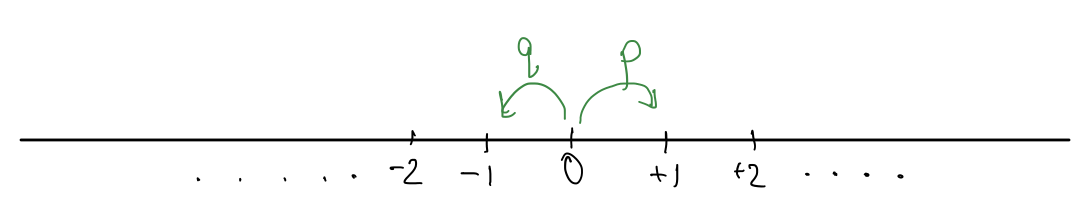
\includegraphics[scale=0.45]{walker_schematic.png}
    \caption{A schematic of random walker defined in one dimension lattice with movement given as +1 step with probability $p$ or a step of -1 with probability $1-p$ or $q$.}
    \label{fig:my_label}
\end{figure}

% Position of walker at $t=0$ is position at $m=0$. After a fixed interval of time , $\Delta t$, the walker is independent to go left or right with probability of $q$ or $p$ respectively where $p+q=1$. 

% \subsection{What do we aim}


% A general random walk graphically, for $1D$ is as depicted in figure below \\
% \begin{figure}[H]
%     \centering
%     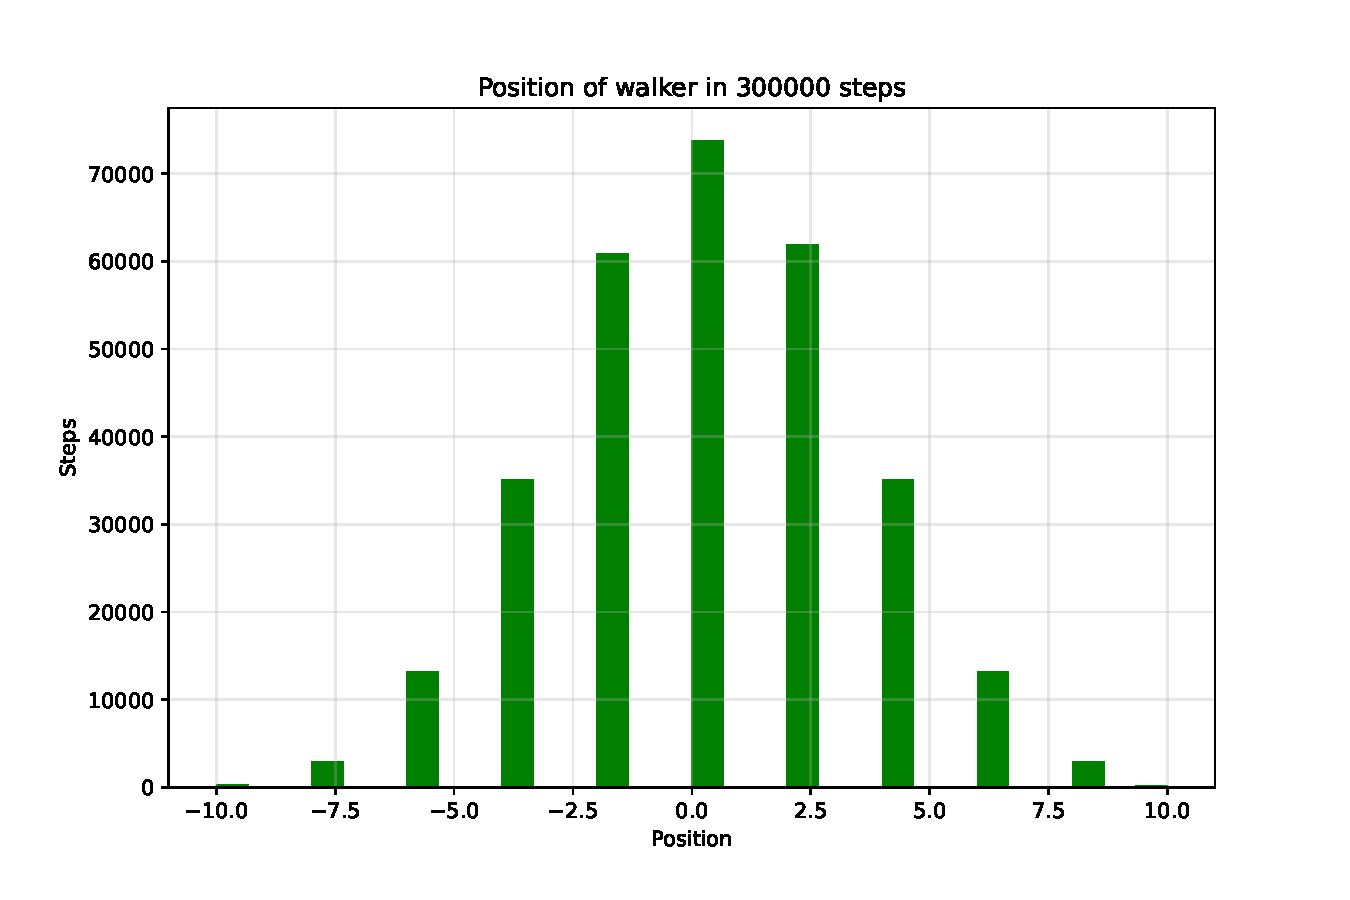
\includegraphics[scale=0.35]{walker.pdf}
%     \caption{A random walk of $300000$ steps. As the maths suggest, we get the mean position around $0$. The abscissa denotes the distance $m$ from the initial position of particle i.e $x=0$ and ordinate axis gives us the probability of finding the particle at that distance $m$ }
%     \label{fig:my_label}
% \end{figure}

% We shall now understand how the Binomial distribution for the walker is spread and how with increasing number of steps the $FWHM$ keeps getting lesser.This will help us understand how and why the Gaussian behaviour gets more apparent with larger steps, $m$ 
% \begin{figure}[H]
%     \centering
%     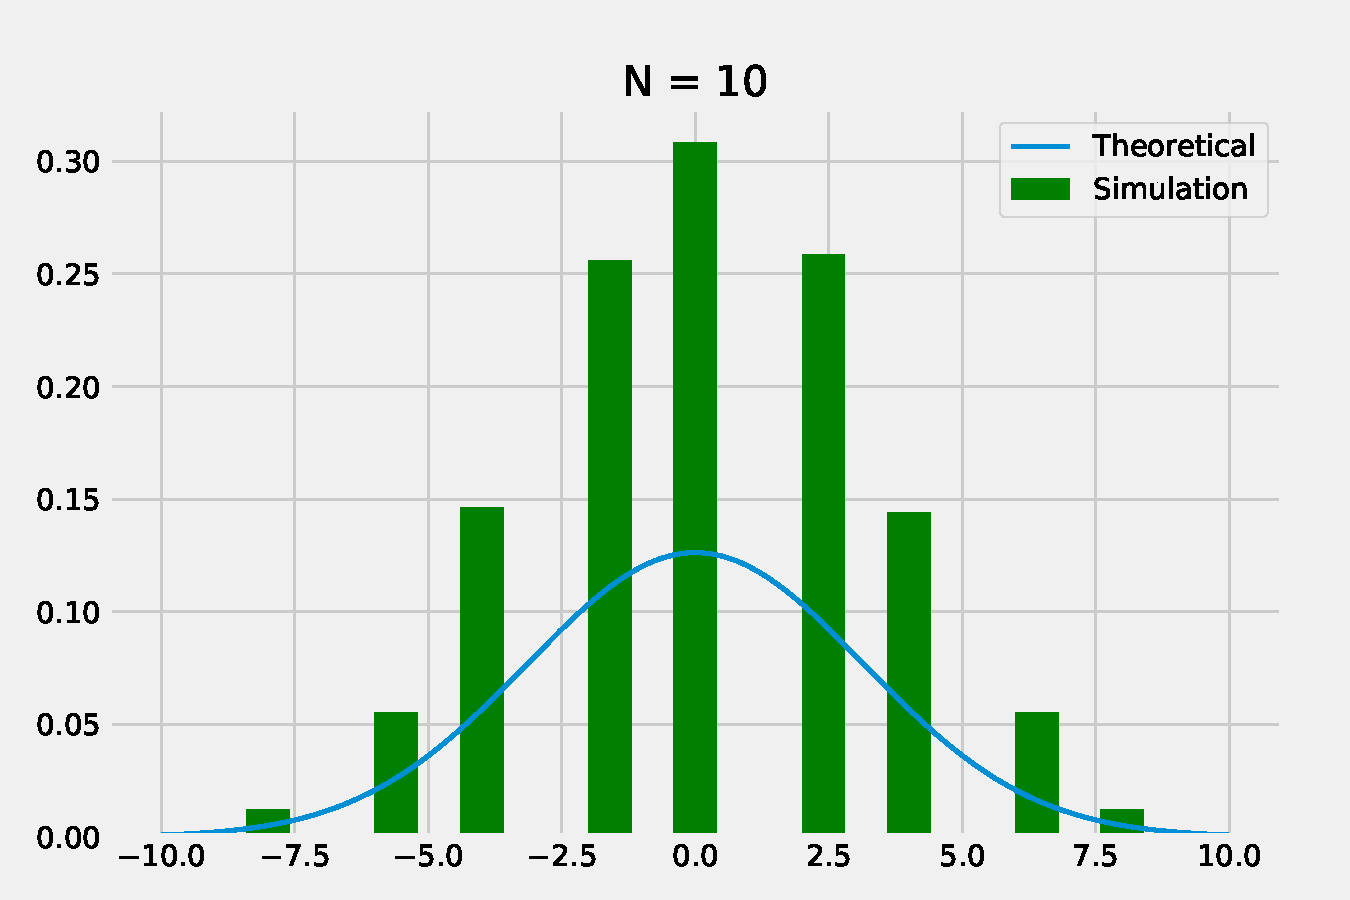
\includegraphics[scale=0.35]{N_10.pdf}
%     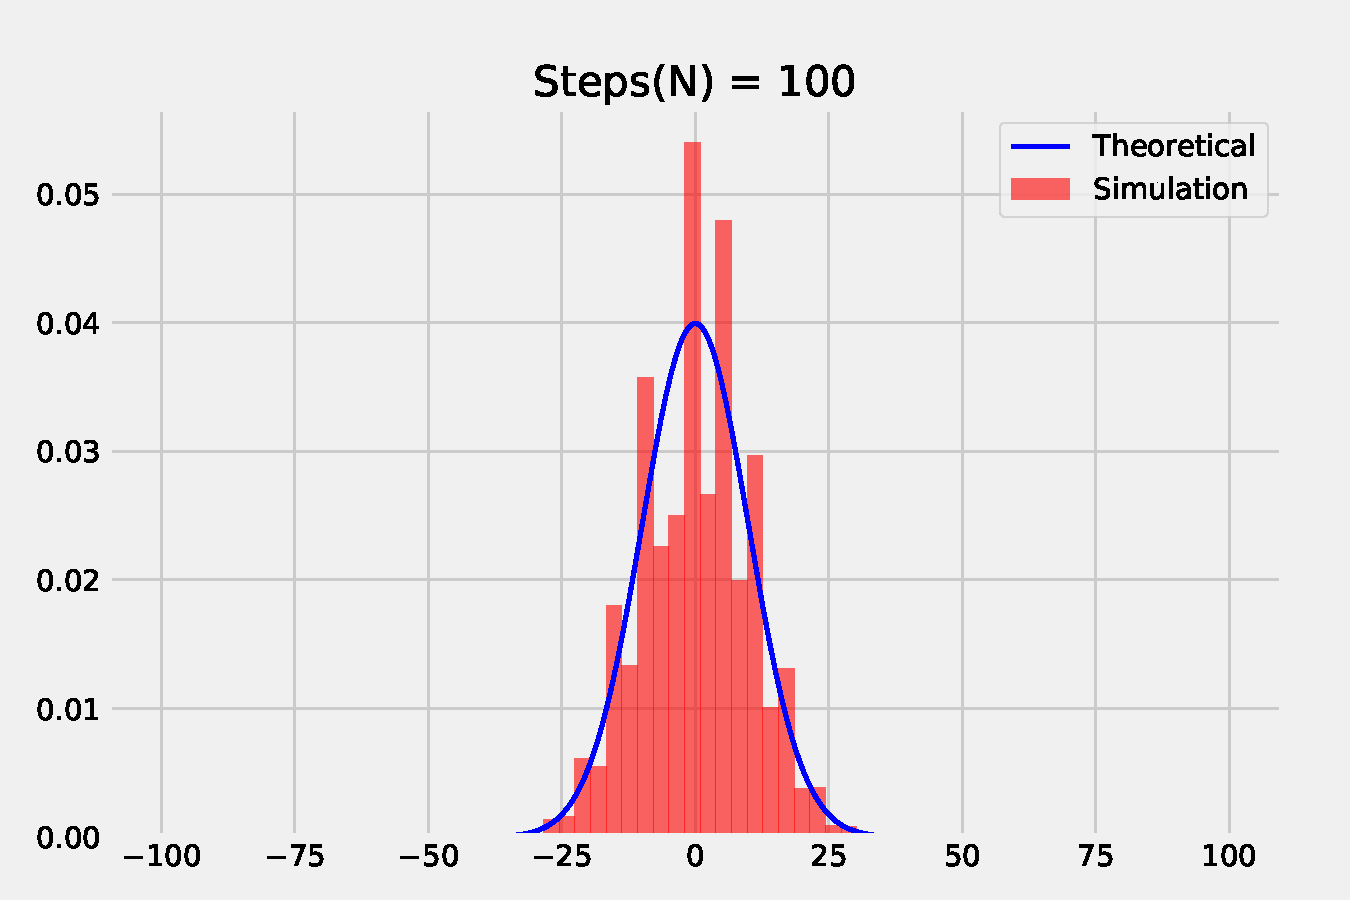
\includegraphics[scale = 0.35]{N_100.pdf}
%     \caption{Theory and Simulation. We observe how the plots get refined with increasing number of steps. Position of walker essentially, at whole depicted by the distribution in the latter figure whereas in the former figure, the distribution does not gives us the accurate answers.}
%     \label{fig:my_label}
% \end{figure}

% Therefore, our aim is to answer the question of -- what is the probability $p(m,N)$ that the walker will be at $m$ step point after taken $N$ steps ? 

\noindent
We are interested in the following question -- what is the probability $p(m,N)$ that the walker will be at $m$ step point after taken $N$ steps ? To answer this question, let us denote
$N = n_1 + n_2$ as the total number of steps taken where
$n_1 = \frac{1}{2}(N + m)$ are jumps to the right and
$n_2 = \frac{1}{2}(N - m)$ are jumps to the left. Therefore, the net displacement , $m$ becomes $m = n_1 - n_2$.



Since the left-right jumps are independent of each other, the probability for making $n_1$ jumps to right and $n_2$ jumps to the left is given by
\begin{align}
    p^{n_1}q^{n_2} = p^{\frac{1}{2}(N+m)}q^{\frac{1}{2}(N-m)}
\end{align}

\begin{figure}[H]
    \centering
    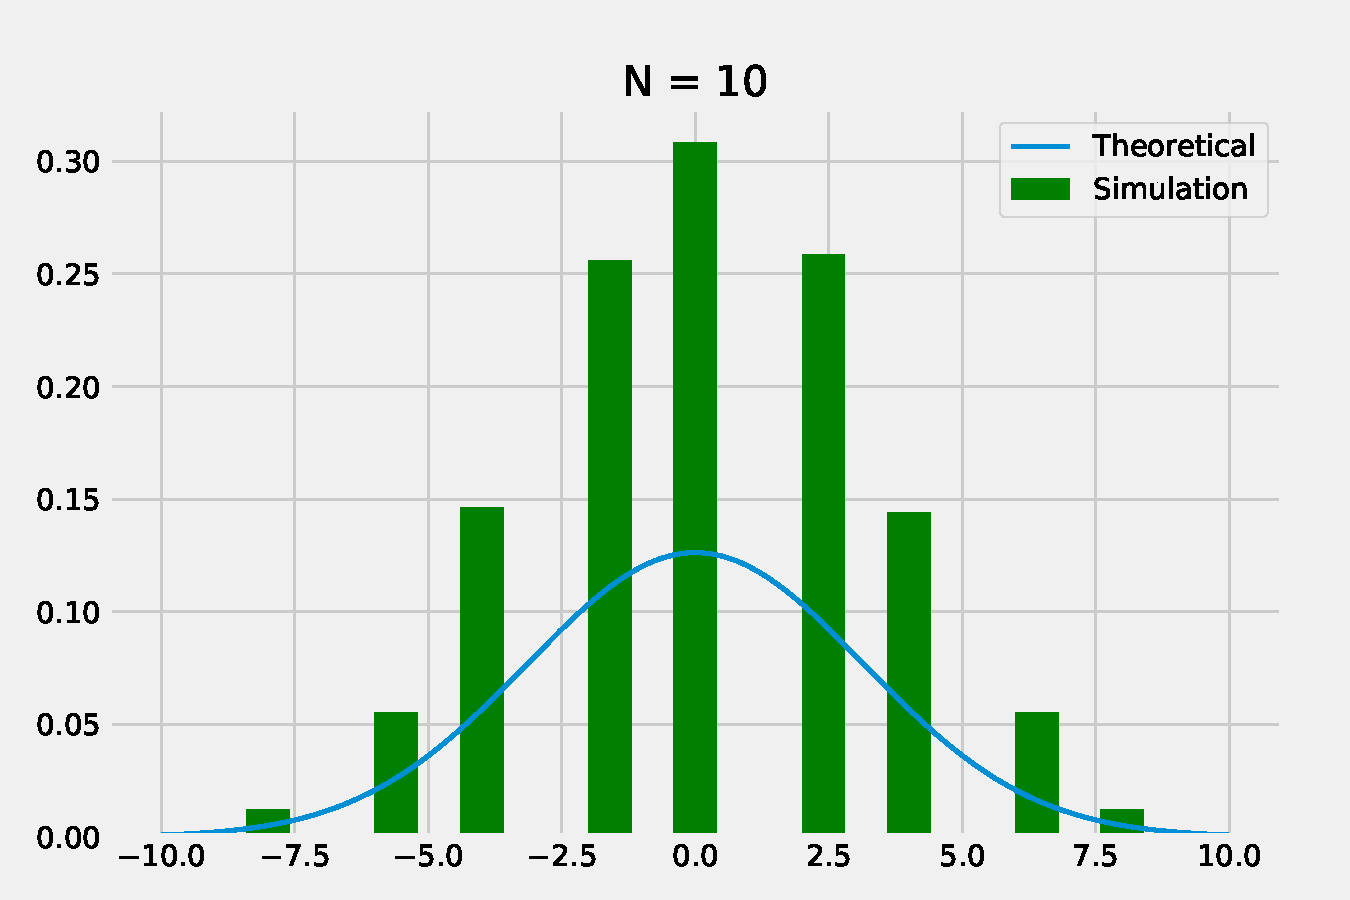
\includegraphics[scale=0.35]{N_10.pdf}
    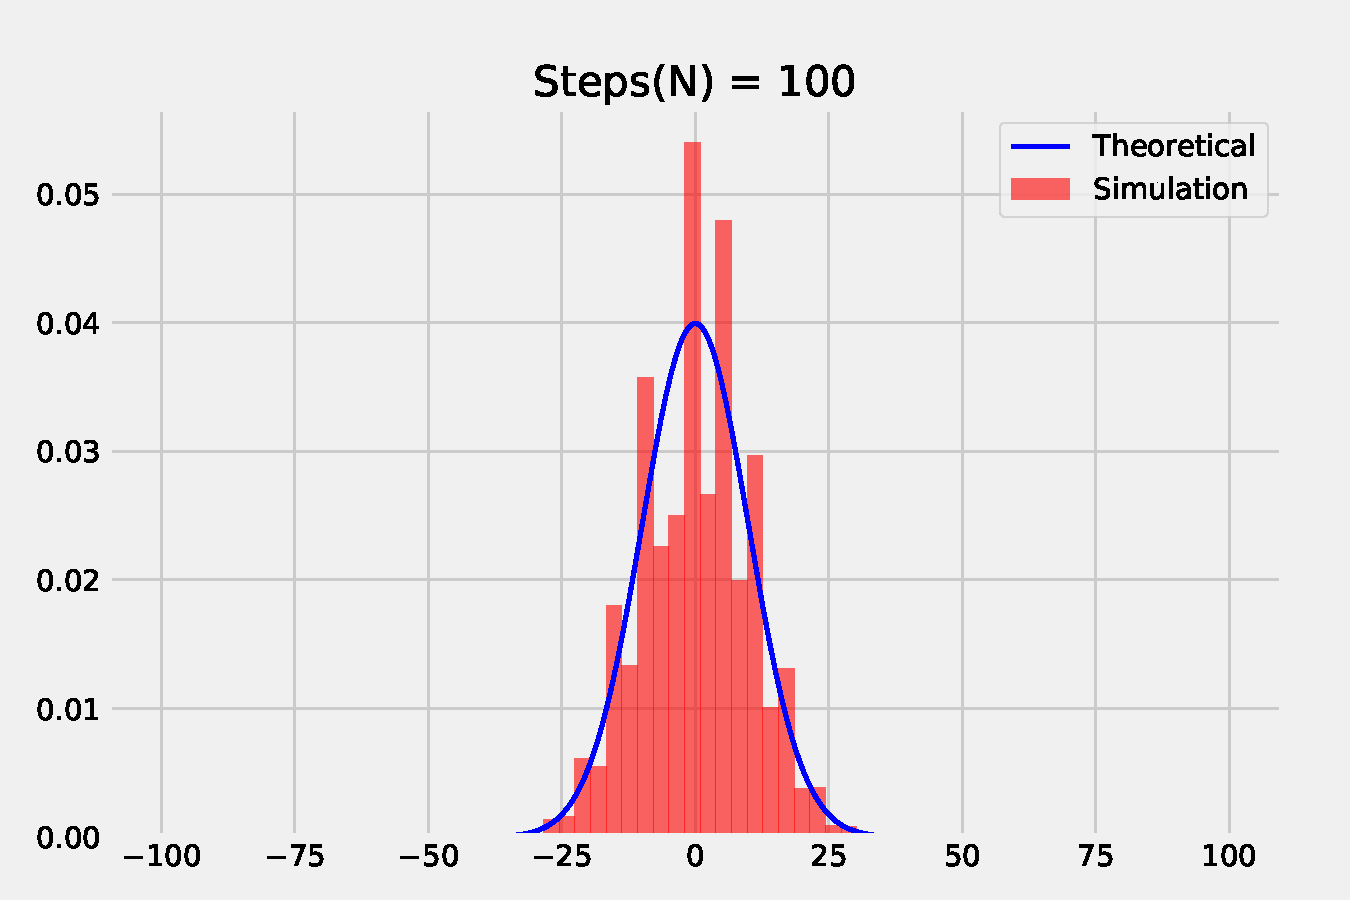
\includegraphics[scale = 0.35]{N_100.pdf}
    \caption{Theory and Simulation. We observe how the plots get refined with increasing number of steps. Position of walker essentially, at whole depicted by the distribution in the latter figure whereas in the former figure, the distribution does not gives us the accurate answers.}
    \label{fig:my_label}
\end{figure}

%As discussed, we simulated the walker and obtained a Gaussian distribution. For increased number of steps, we start to see a lesser spread distribution. Referring to Fig. 2, we can duly observe the difference in distribution with increased number of walker

Let us now compute the total number of paths
made by the walker in $N$ steps. The first object of the jumps can be chosen in $N$ ways, later the $(N-1)$ , then $(N-2)......(N-n_1 - 1)$ ways.\\So, the total number of distinguishable ways to have $n_1$ steps to the right and $n_2$ to the left will be 
\begin{align}
    \frac{N!}{n_1 !}  =  \frac{N!}{n_1 ! (N-n_1)!}
\end{align}

So, therefore the probability of being at at position $m$ after $N$ jumps or notably $p(m,N)$ is
\begin{align}
    p(m,N) = \frac{N!}{(\frac{N+m}{2})! (\frac{N-m}{2})!} p^{\frac{1}{2}(N+m)} q^{\frac{1}{2}(N-m)}
\end{align}

Devising the equation for number of steps to the right , 
\begin{align}
n \equiv n_1 = \frac{N+m}{2}\\
p(m,N) = p_N(n) = \frac{N!}{n!(N-n)!}p^n q^{N-n}\\
P_N(n) = \binom{N}{n} p^n q^{N-n}
\end{align}
which is verified in Fig. 2.


\subsection{Moments of the displacement for the random Walk}
We can calculate all moments of $n$ at any fixed time $N$ since we know the probability distribution $p(m,N)$ from Eq. (6). For first moment, we have 
\begin{gather}
    n p^n = p \frac{\partial}{\partial p}(p^n)\\
\langle n \rangle=    \sum_{n=0}^{N} n p^n q^{N-n},\\
    \sum_{n=0}^{N} \binom{N}{n} p \frac{\partial}{\partial p} (p^n) q^{N-n}\\
    p \frac{\partial}{\partial p} \sum_{n=0}^{N} \binom{N}{n} p^n q^{N-n}\\
    p \frac{\partial}{\partial p} (p+q)^N = Np(p+q)^{N-1} = Np
\end{gather}

Further for second moment, 
\begin{gather*}
\langle n^2 \rangle=    \sum_{n=0}^{N} n^2 p_N(n) = \sum n• \underbrace{\big<n•p_N(n)\big>}_A
\end{gather*}

and we already have derived the value to the quantity $A$, 
\begin{gather*}
    \sum_{n=0}^{N} n^2 p_N(n) = n \frac{\partial}{\partial p} \sum_{n=0}^{N} \binom{N}{n} p^n q^{N-n} p \frac{\partial}{\partial} p^n
    \\p \frac{\partial}{\partial p} (p+q)^N  = p \frac{\partial}{\partial p} \big( Np + (p+q)^{N-1} \big)\\
    =(Np) + \bigg(N-1)Np^2\bigg)
\end{gather*}


%The distribution attains a bell shaped form with a $maximum$ occurring around average value $<n>=Np$.

%Now, getting a little back, we can now write the $p_N(n)$ , position of walker after N steps, 
Moments for the displacement simply reads
\begin{align}
    <m> = 2<n> - N = N(p-q)
\end{align}

and for second moment , 
\begin{align}
    <m^2> = 4<n^2> - 4<n>N + N^2
\end{align}

Variance of displacement, 
\begin{equation}
    \sigma_m ^2 = 4\sigma^2 = 4Npq,
\end{equation}
which is verified in Fig. 3.
\newline

% \begin{figure}[H]
%     \centering
%     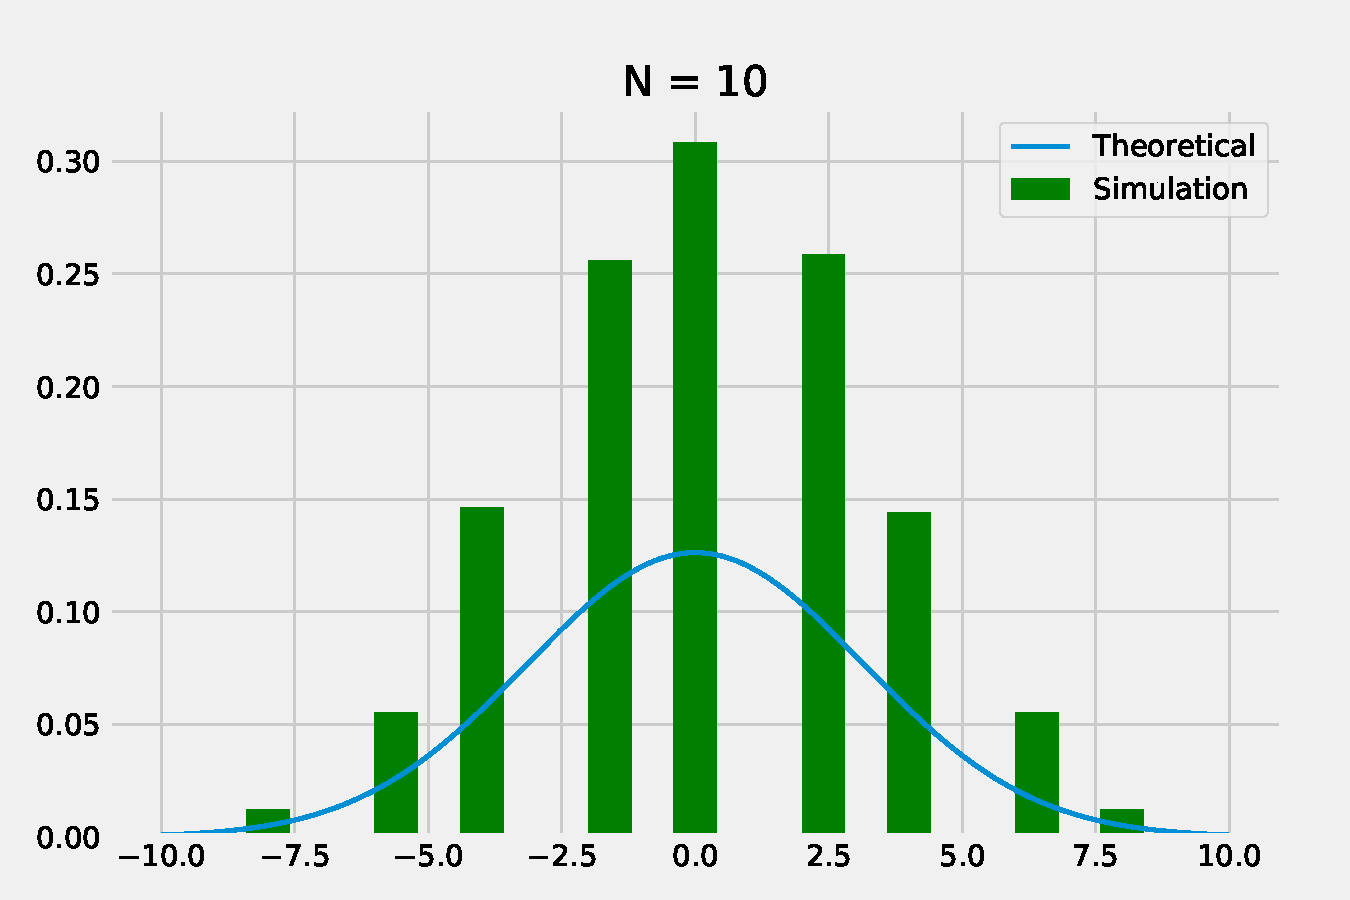
\includegraphics[scale=0.35]{N_10.pdf}
%     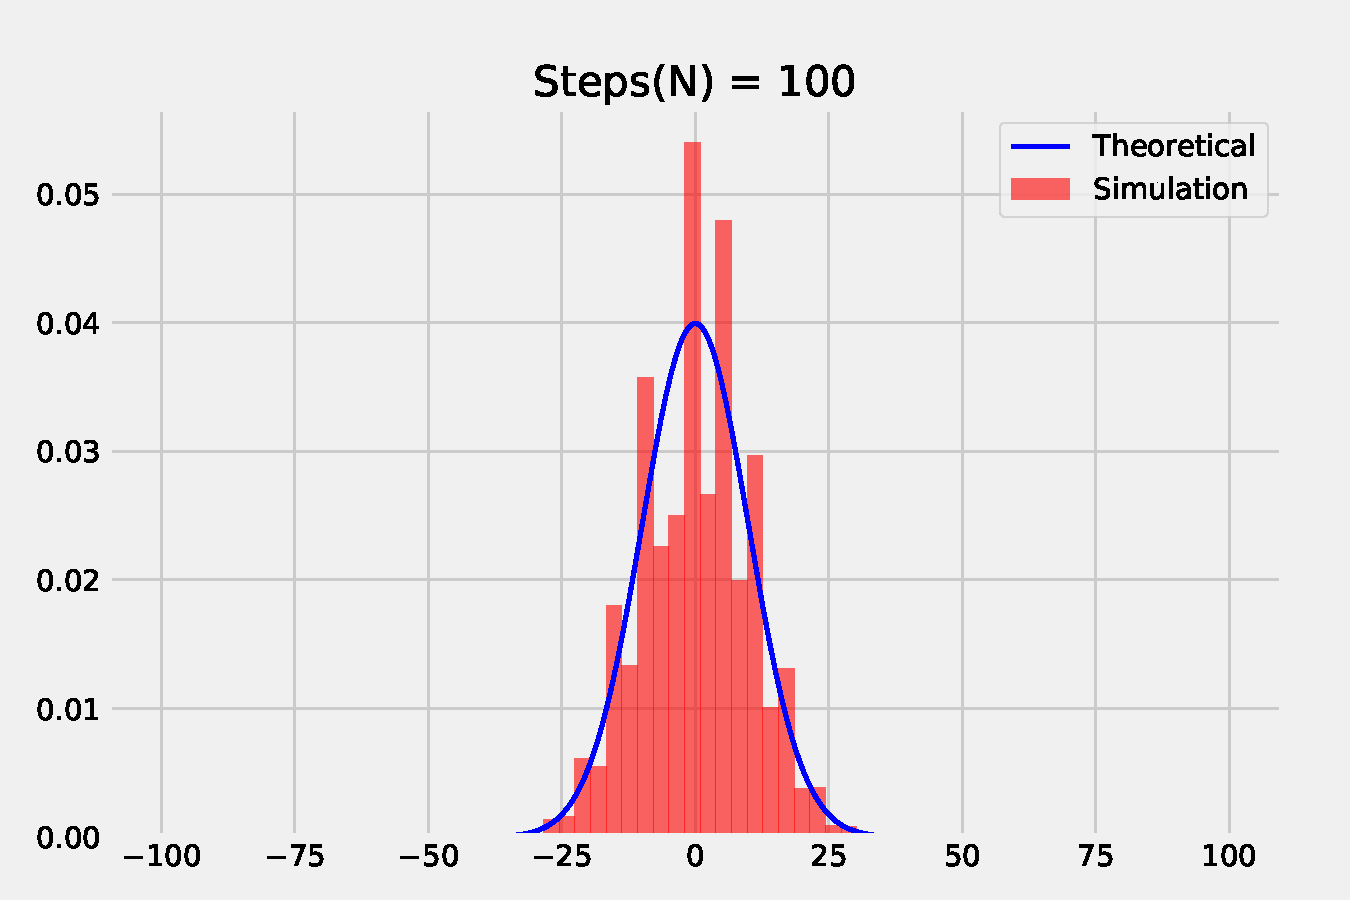
\includegraphics[scale = 0.35]{N_100.pdf}
%     \caption{Theory and Simulation. We observe how the plots get refined with increasing number of steps. Position of walker essentially, at whole depicted by the distribution in the latter figure whereas in the former figure, the distribution does not gives us the accurate answers.}
%     \label{fig:my_label}
% \end{figure}

% As discussed, we simulated the walker and obtained a Gaussian distribution. For increased number of steps, we start to see a lesser spread distribution. Referring to Fig. 2, we can duly observe the difference in distribution with increased number of walker


% \subsection{Biased or Asymmetric walker}

% We derived the mean for the symmetric walker to be $ \mu = 0$ as $p=q = 0.5$ and mean was derived by $N(p-q)$.\\
% This , therefore, becomes intuitive that when $p \neq q$ , then $\mu \neq 0$. There will a shift of the distribution on position axis. The result were as shown by figure below 




%We have so far observed the Gaussian distribution for the different number of steps will vary. The mathematical conclusion for the same can be analyses by mean square displacement. This computational analysis will provide us with the answer how far the walker will have traveled in the given number of steps. We will simply need single set of data for this purpose , namely trajectory of the walker with time. Since ,we are taking $\delta t$ = 1 for difference between each step, our formula for MSD reduces to \\
%\begin{gather}    MSD(\tau = 1) = {\big< \big( x(t + \tau) - x(t) \big)^2 \big>}
%\end{gather}


%This gives us the idea how much area the particle would have covered in given $\tau$ steps. As we would expect, the graph that we get is linear as the walker is without resetting - the simple random walk. \\


\begin{figure}[H]
    \centering
    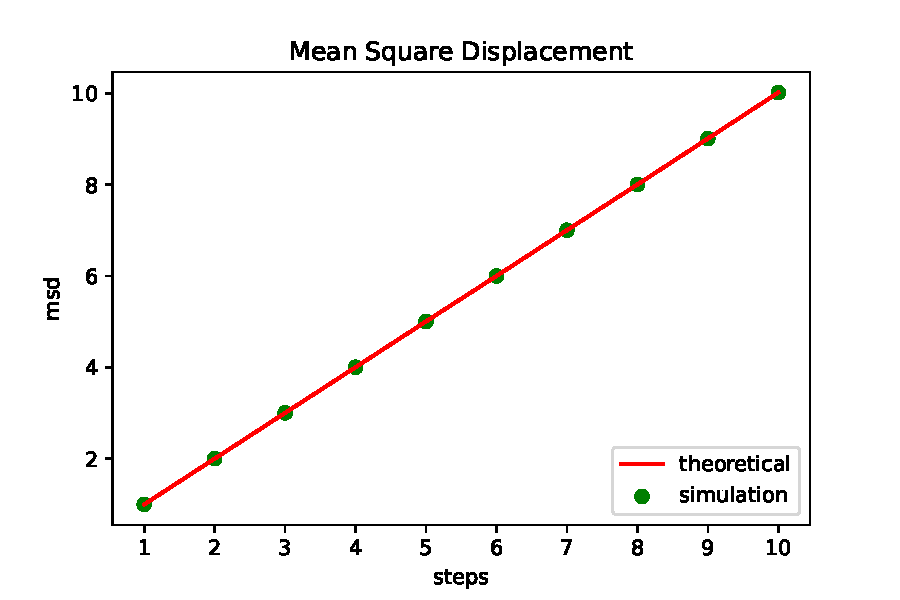
\includegraphics[scale=0.60]{msd.pdf}
    \caption{Mean Square Displacement for given walker with 10 steps. As is the case for simple random walker ($p=q=0.5$) we get a linear dependence.}
    \label{fig:my_label}
\end{figure}

%We will further see how when a resetting is introduced to the walker, the plot starts to perturb signifying the walker is essentially within a confinement and for large number of steps, the plot starts to stay irrespective of the number of steps.
We plot the $MSD$ as a function of $N$ in Fig. 3. We see a perfect match between the theoretical and simulation result. %As we can infer from Eq. 14 that , it reduces to $4Npq$ which infact gives a linear plot as we observe .



\subsection{Arguments based on the Central Limit Theorem }

% \subsection{Moments of Walks}

% We can calculate all moments of $m$ at any fixed time $N$ if we know the probability distribution $p(m,N)$. \\ For first moment ,we have, 
% \begin{gather*}
%     n p^n = p \frac{\partial}{\partial p}(p^n)\\
%     \sum_{n=0}^{N} n p^n q^{N-n},\\
%     \sum_{n=0}^{N} \binom{N}{n} p \frac{\partial}{\partial p} (p^n) q^{N-n}\\
%     p \frac{\partial}{\partial p} \sum_{n=0}^{N} \binom{N}{n} p^n q^{N-n}\\
%     p \frac{\partial}{\partial p} (p+q)^N = Np(p+q)^{N-1} = Np
% \end{gather*}

% Further for second moment, 
% \begin{gather*}
%     \sum_{n=0}^{N} n^2 p_N(n) = \sum n• \underbrace{\big<n•p_N(n)\big>}_A
% \end{gather*}

% and we already have derived the value to the quantity $A$, 
% \begin{gather*}
%     \sum_{n=0}^{N} n^2 p_N(n) = n \frac{\partial}{\partial p} \sum_{n=0}^{N} \binom{N}{n} p^n q^{N-n} p \frac{\partial}{\partial} p^n
%     \\p \frac{\partial}{\partial p} (p+q)^N  = p \frac{\partial}{\partial p} \big( Np + (p+q)^{N-1} \big)\\
%     (Np) + \bigg(N-1)N(p^2)\bigg)
% \end{gather*}

% {Various other moments of $N$},
% \begin{itemize}
%     \item $E[n] = <n> = Np$
%     \item $E[n^2] = <n^2> = Np + N(N-1)p^2$
% \end{itemize}
% \begin{center}
%     $Var[n] = \sigma^2 = <n^2> - <n>^2$\\
%     $Np + N(N-1)p^2 - (Np)^2$\\
%     $= Npq$
% \end{center}

% The distribution attains a bell shaped form with a $maximum$ occurring around the average value $<n>=Np$

% Now, getting a little back, we can now write the $p_N(n)$ , position of walker after N steps, 
% \begin{align}
%     <m> = 2<n> - N = N(p-q)
% \end{align}

% and for second moment , 
% \begin{align}
%     <m^2> = 4<n^2> - 4<n>N + N^2
% \end{align}

% Variance of displacement, 
% \begin{equation}
%     \sigma_m ^2 = 4\sigma^2 = 4Npq
% \end{equation}
% \newline

% \subsection{Biased or Asymmetric walker}

% We derived the mean for the symmetric walker to be $ \mu = 0$ as $p=q = 0.5$ and mean was derived by $N(p-q)$.\\
% This , therefore, becomes intuitive that when $p \neq q$ , then $\mu \neq 0$. There will a shift of the distribution on position axis. The result were as shown by figure below 







% \subsection{For larger number of steps}

We observed that PDF ($p_m(N)$) for 1D walker is exactly Binomial Distribution. But when we start to increase the number of walkers, we start to observe some really interesting results. This can be seen in Fig. 2 and Fig. 4.
% We observe that for larger number of steps of walker,  we start to see a Gaussian behaviour in the distribution.\\
We now will understand the math behind this Gaussian behavior. 
First we note that, motion of a RW(random walker) can be written as \\
\begin{align}
    x_n = x_{n-1} + \zeta _n
\end{align}
where $\zeta _n$ is a random variables defined as 
\begin{align}
\zeta _n =\begin{cases}
          +1 \quad & \,  \textnormal{with prob p} \\
          -1 \quad & \,  \textnormal{with prob q}  \\
     \end{cases}
\end{align}
equivalently writing, to note $p(\zeta)$ has the following PDF
\begin{align}
    p(\zeta) = p \delta(\zeta -1) + q\delta (\zeta + 1)
\end{align}
Iterating the steps for $n= 0,1,2,...$ we write, 
\begin{align}
    x_1 = x_0 + \zeta _0 \\
    x_2 = x_1 + \zeta _1 \\
    x_2 = x_0 + \zeta _0 + \zeta _1\\
    ....\\
    x_n = x_0 + \sum_{i = 1}^{n-1} \zeta _i
\end{align}
Note that at each step, $\zeta$ is statistically identical and also independent. In other words, $\zeta$ is an $i.i.d$ random variable. 
From the knowledge of central limit theorem, we know that a random variable which is a sum of such random variables will attain to a Gaussian distribution as long as the mean and variance of the parent random variables are finite.
% \begin{align}
%     x_n = \sum_{i = 1}^{n-1} \zeta _i
% \end{align}

This is the reason, we see the distribution converging to a Gaussian. note that, the Gaussianity is observed within the $\sqrt{N}$ width around the mean. Refer Fig. 4. It is crucial to note that this result hold true for any random variable $\zeta$ (independent of any specific form of their PDF) as long as  they remain IID with finite mean and variance.

\begin{figure}[H]
    \centering
    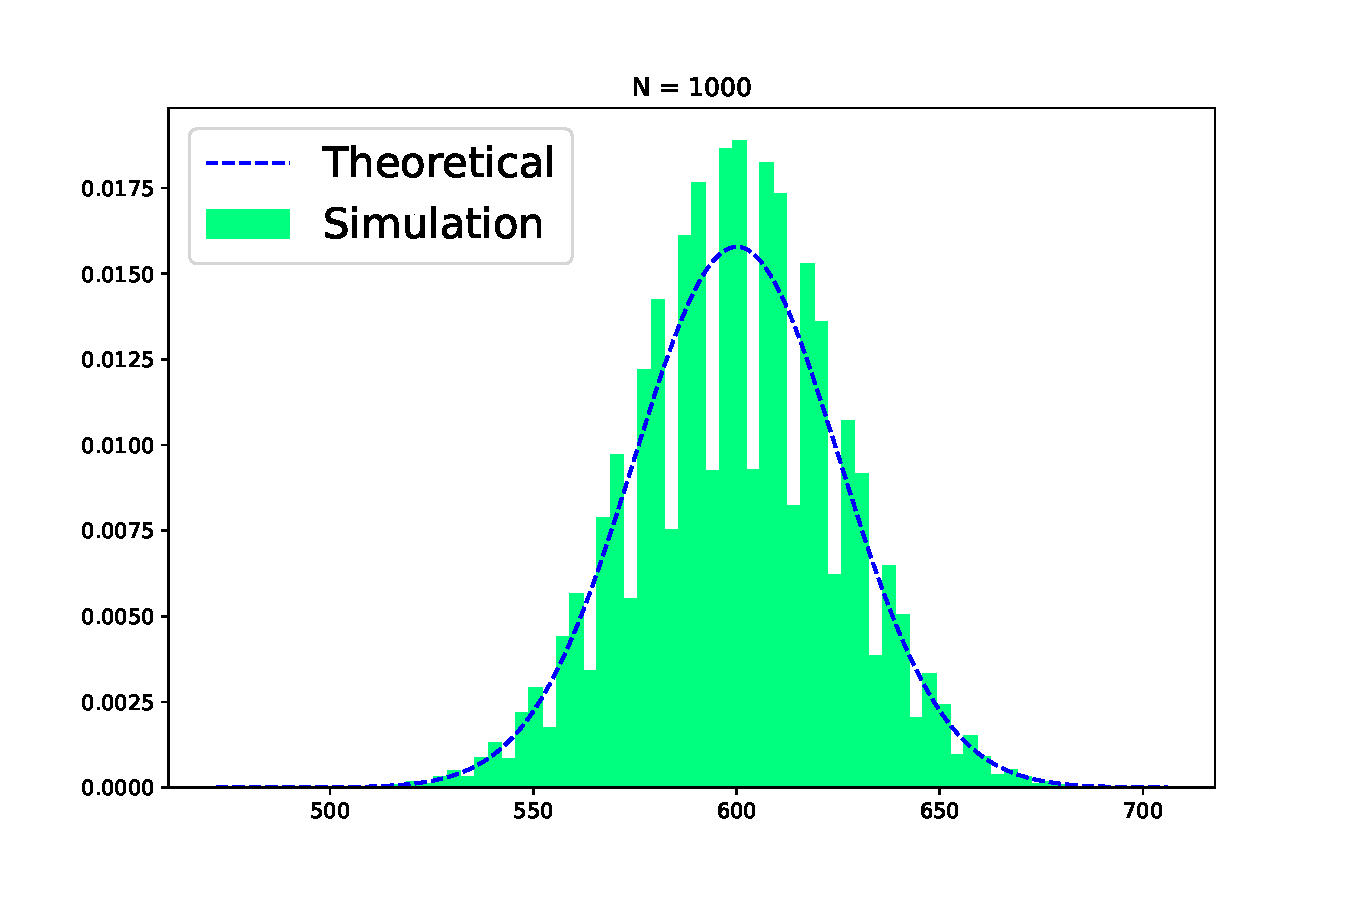
\includegraphics[scale= 0.35]{N_1000_biashed.pdf}
    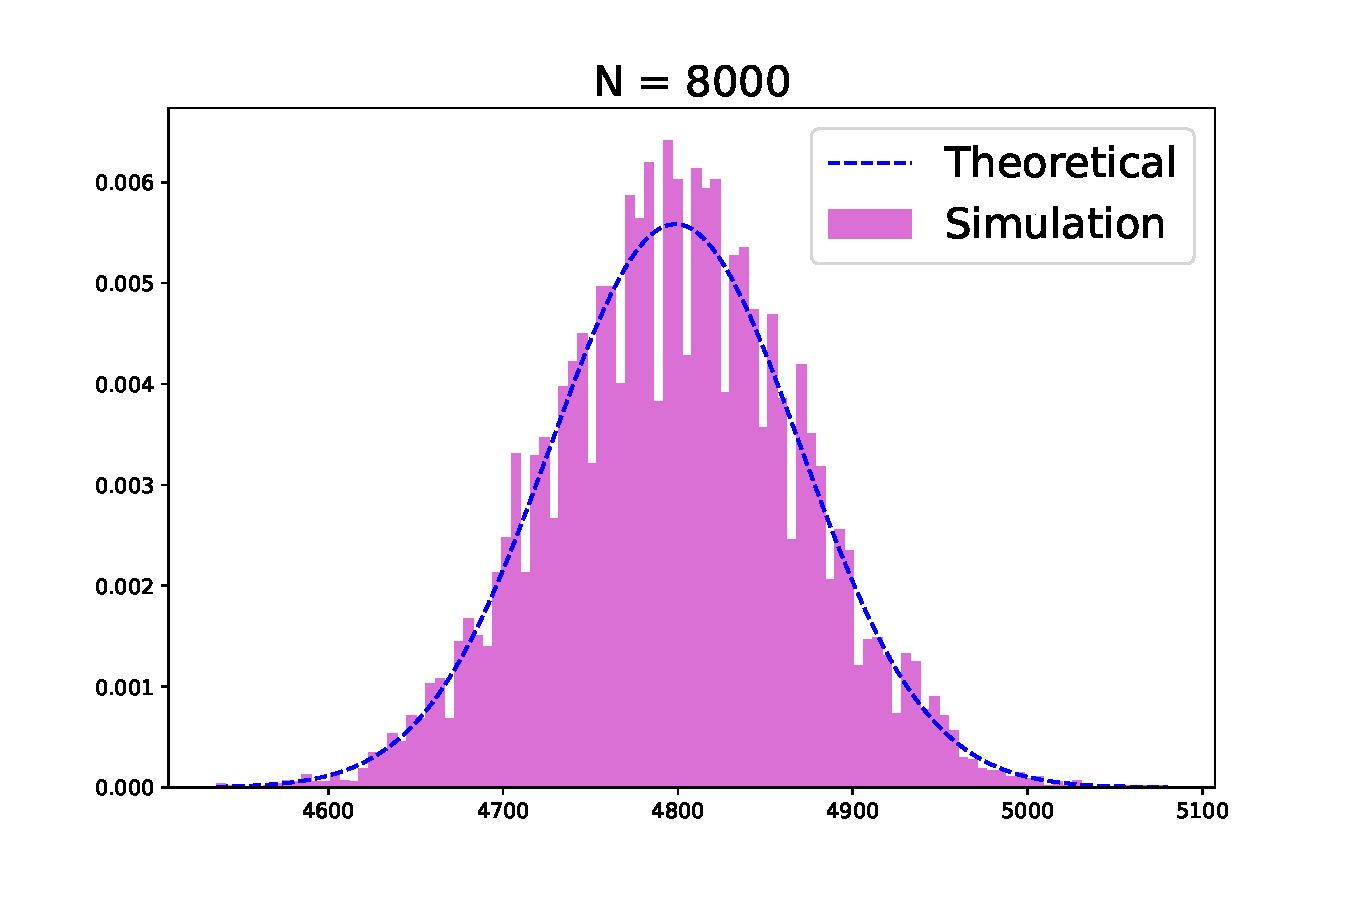
\includegraphics[scale = 0.40]{N_8000_biashed.pdf}
    \caption{Walker with $p = 0.8$ and $q = 0.2$ for $1000$ and $8000$ steps, we continue to get a Gaussian distribution with $\mu$ defined as $N(p-q)$. Our simulations holds good accuracy with the mathematics.}
    \label{fig:my_label}
\end{figure}


% when the number of samples are increased to large numbers, here steps.
% The convergence to Gaussian distribution for $N$ number of steps is limited as per Central Limit Theorem as $ \sqrt{N}$


% width is of order  $ \sqrt{N}$ around the mean --- this is crucial for CLT to hold ... you need a finite mean and variance for the RVs you're adding... 

% \subsection{Symmetric and Asymmetric Walker}

We tested the walker with $p=q= \frac{1}{2}$ and observed that mean tends at $0$ i.e $\mu = 0$ which is in total agreement with the theory. We, likewise obtained a Gaussian distribution.\\ Then we allowed walker with $p \neq q$ and we set $p =0.6$ and $q = 0.4$ and as we would expect the average $\mu \neq 0$ and resultant we observed a rightward shift in the plot as $p>q$
% \\The obtained plots are as shown in figure below. 
% \begin{figure}[H]
%     \centering
%     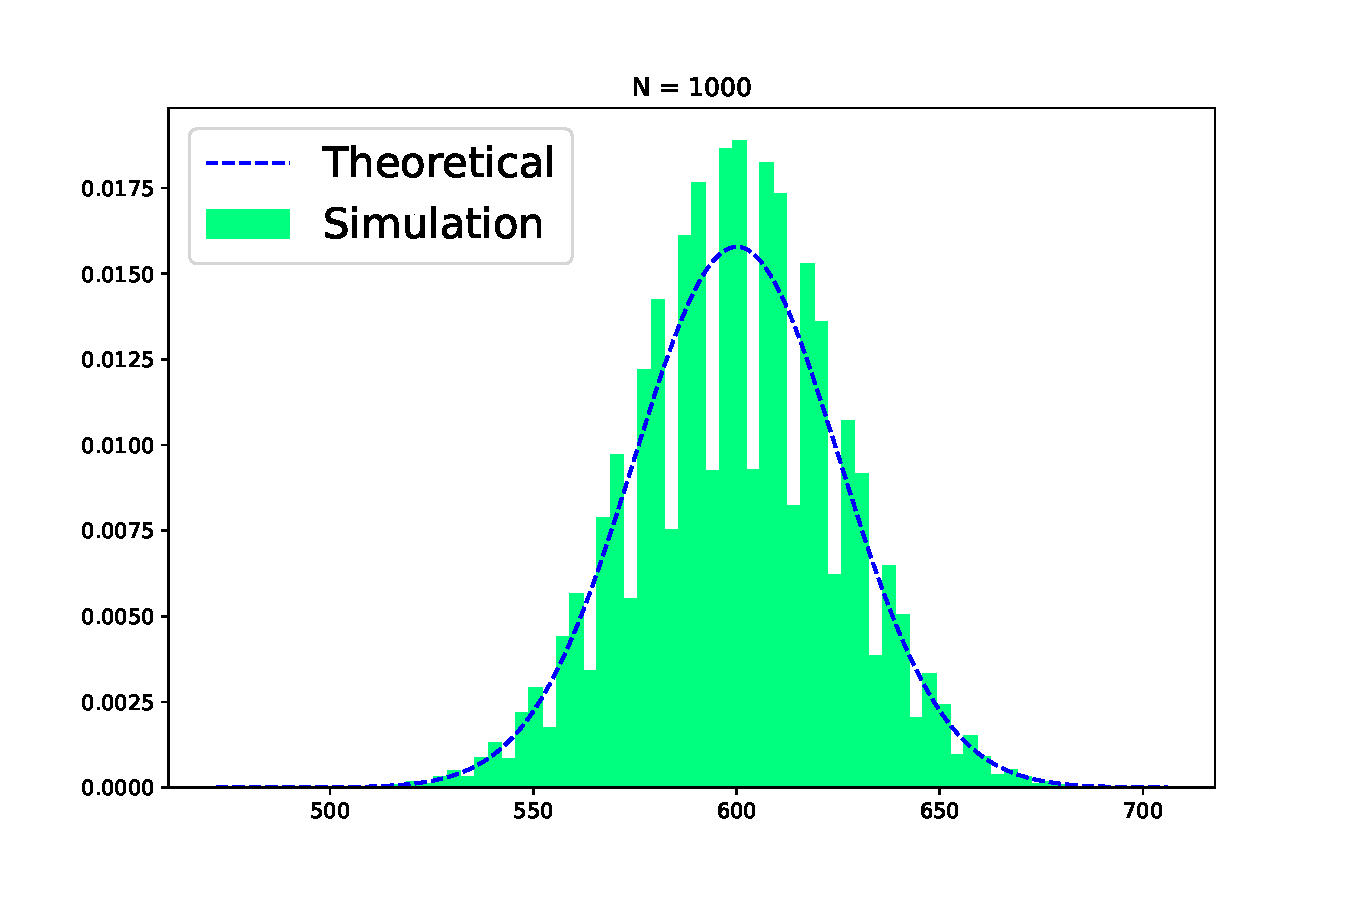
\includegraphics[scale= 0.40]{N_1000_biashed.pdf}
%     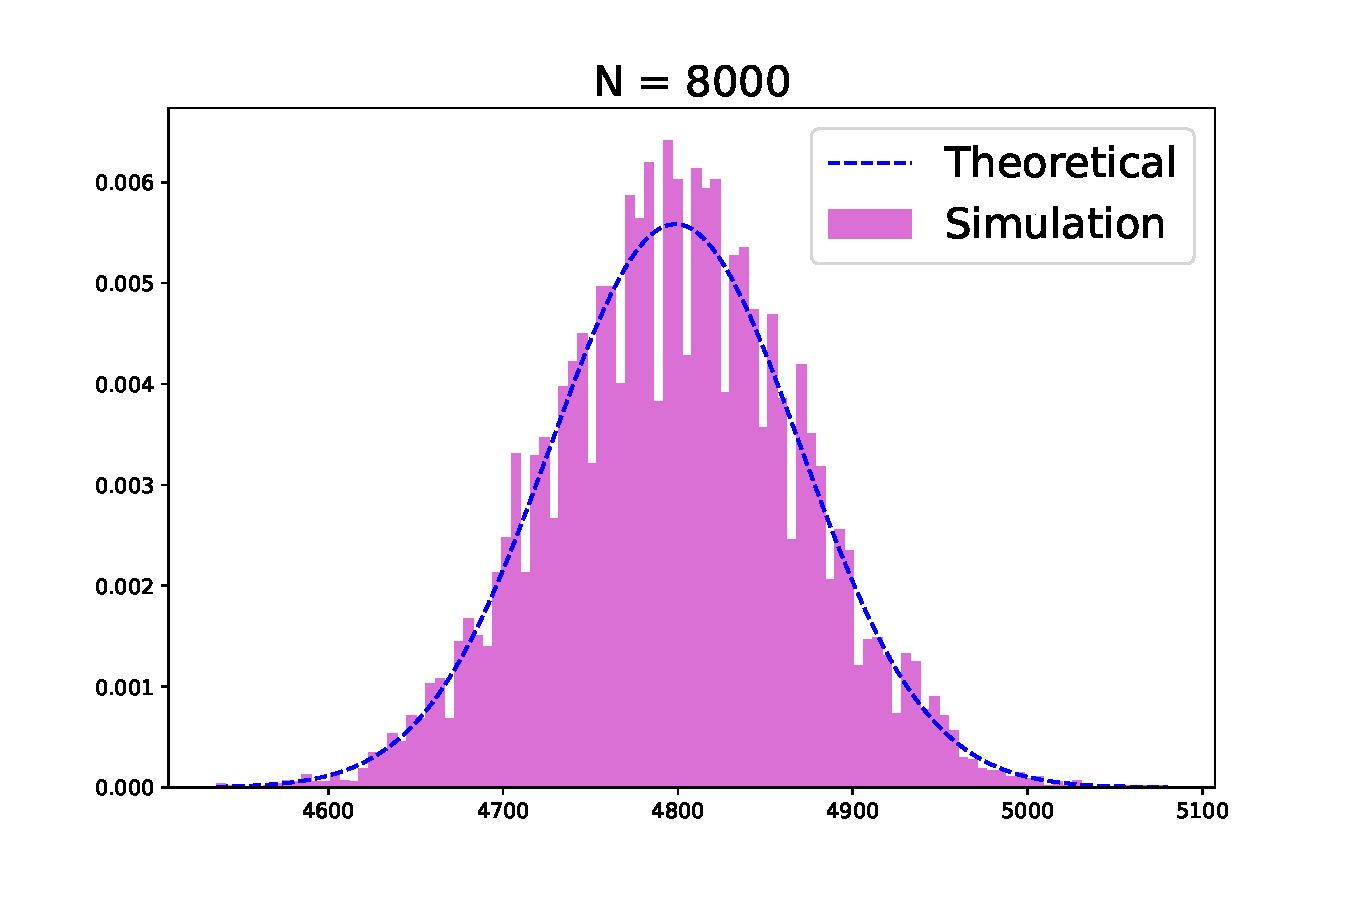
\includegraphics[scale = 0.40]{N_8000_biashed.pdf}
%     \caption{Walker with $p = 0.8$ and $q = 0.2$ for $1000$ and $8000$ steps, we continue to get a Gaussian distribution with $\mu$ defined as $N(p-q)$. Our simulations holds good accuracy with the mathematics.}
%     \label{fig:my_label}
% \end{figure}

\section{Resetting walker}

In this section, we discuss the resetting walker.We allow the walker to restart the whole process for certain probability $r$. By 'resetting', we mean to relocate the walker instantly to the initial position and the process restarts from there.

% Graphically , we start to observe that plots cease to be Gaussian and for larger steps, plots remain no longer differential. As suggested theoretically, the mean, $\mu$ gets shifted.

To note, when we say the walker is reset the $x_r$, we explicitly intend that walker have no memory of past walk. Else, if such conditions are not met, we can not ignore the previous walk after each resetting. This the necessary condition for resetting.
% To demonstrate this condition, we can define a walker with property $f(t) = t$ and $x(t) = t$. We will clearly notice that for each reset, the walker will be put to $x_r = x_0 = 0$ but the $f(t)$ property of walker continues to be carried onward from each journey and it keeps continuing linearly.
% The results obtained is shown in figure below.
\begin{figure}[H]
    \centering
    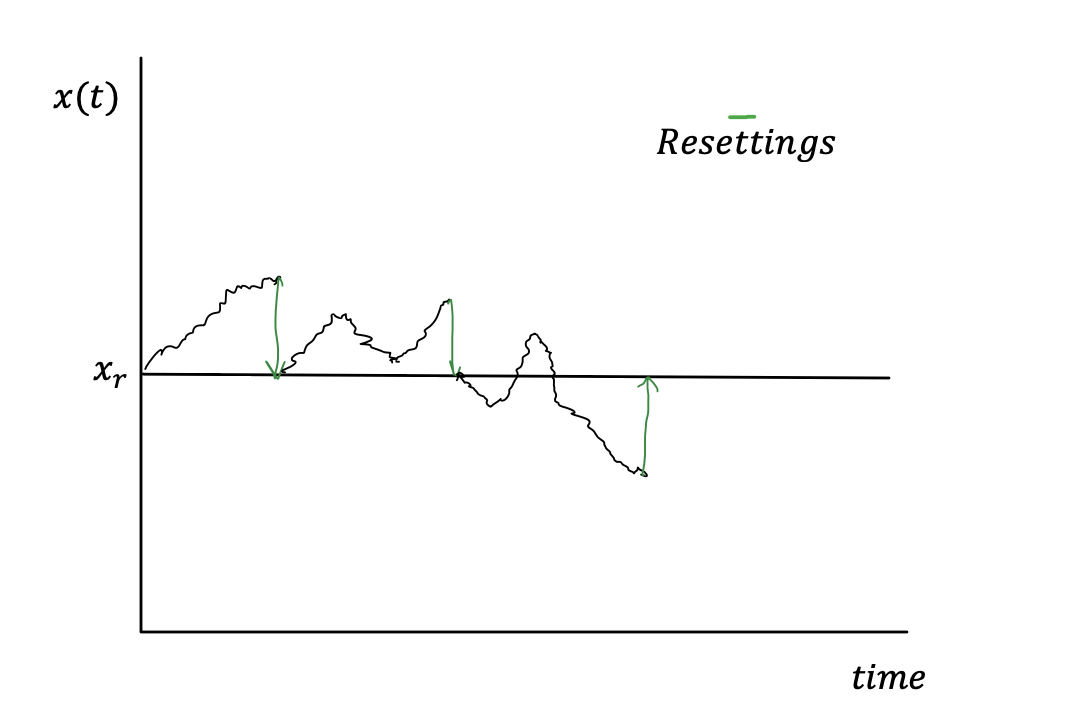
\includegraphics[scale=0.45]{resetting.png}
    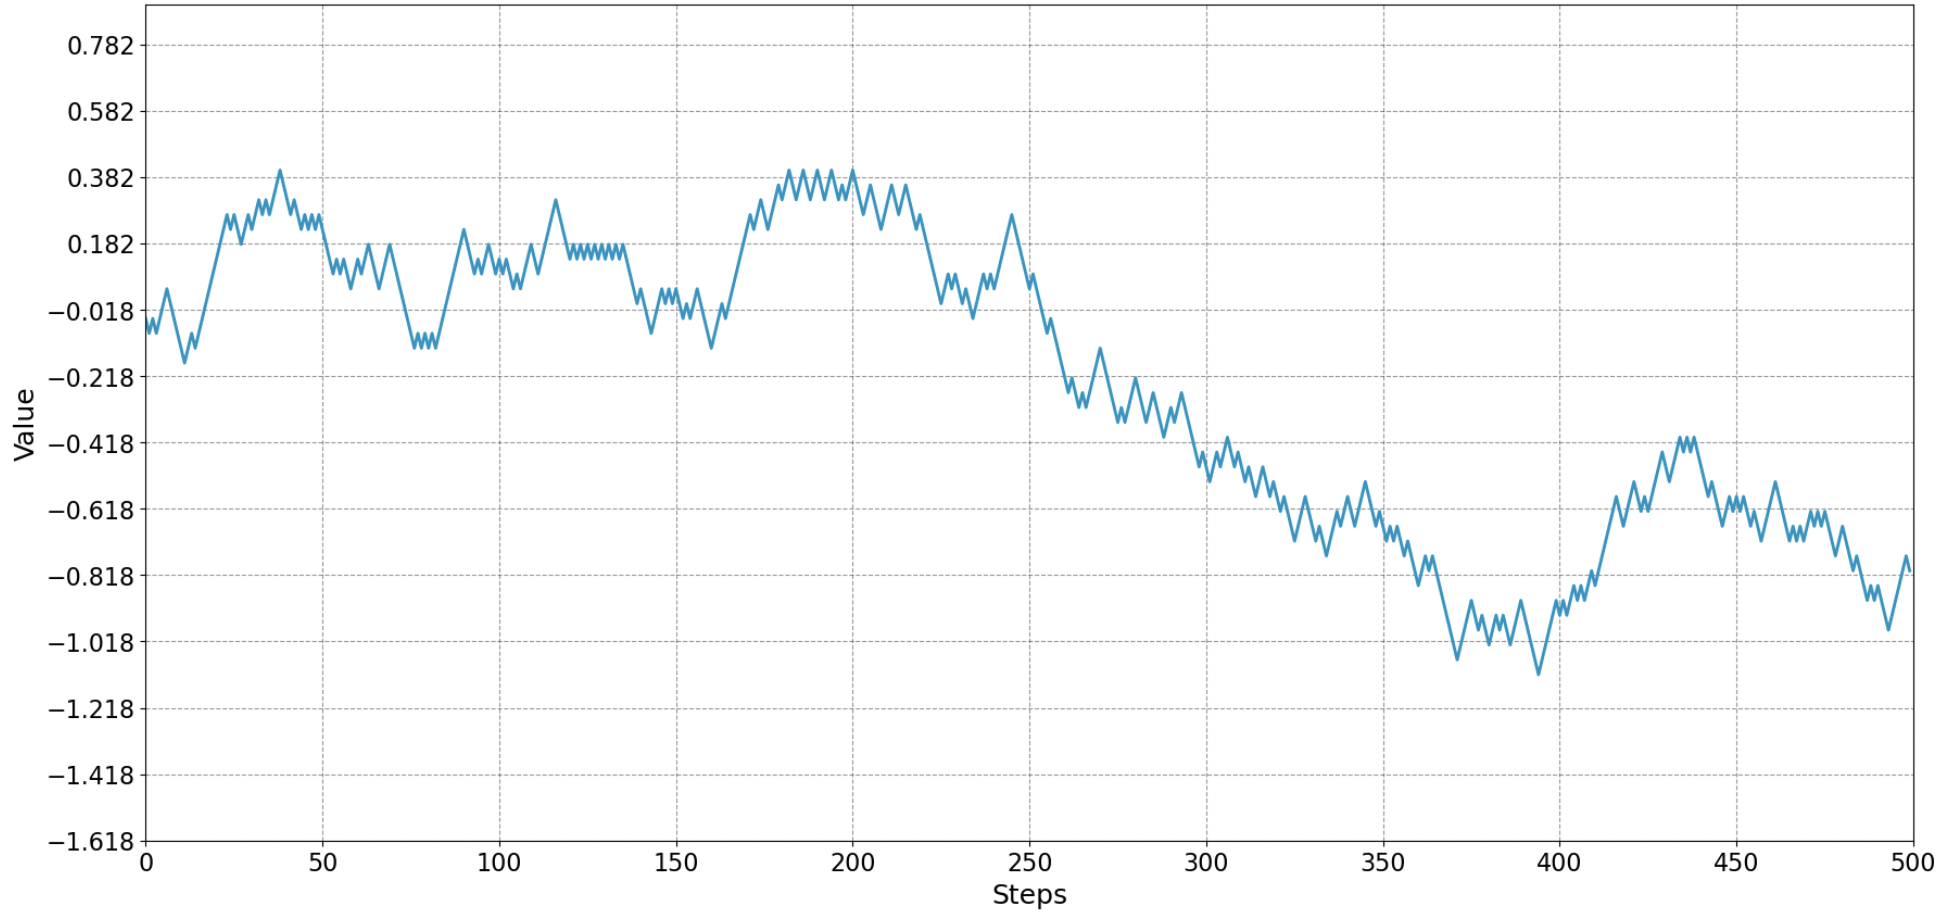
\includegraphics[scale = 0.25]{steps.png}
    % 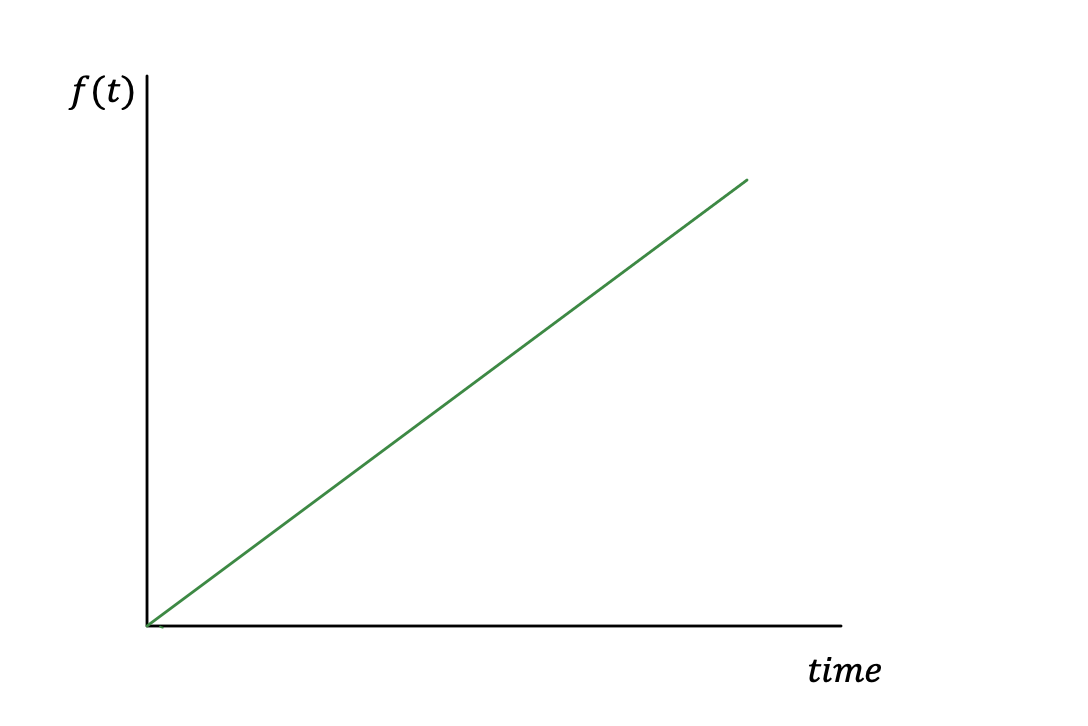
\includegraphics[scale = 0.35]{f(t).png}
    \caption{A schematic of walker with resetting (above) and resetting-less (below) events.}
    \label{fig:my_label}
\end{figure}

So, for resetting walker, we can define the governing equation for the position of the walker as

\begin{align}
x_{n+1} =\begin{cases}
          x_r \quad & \,  \textnormal{with probab r} \\
          x_n + \zeta _n \quad & \,  \textnormal{with probab 1-r}
     \end{cases}
\end{align}
i.e., with probability $r$, the walker is reset to $x_r$ independent of its current location. Otherwise, it makes the random moves.
\subsection{Governing Equations for the PDF}
To write the governing time dependent equations for the PDF, we first observe that the walker erases its memory after each resetting event. In other words, resetting mechanism makes the intervals between any two reset events independent from each other. This is a crucial observation that helps us reduce the problem to great extent. Provided that $n$ resetting happens (note that at least $1$ resetting should happen for this approach), we can have the advantage of eliminating all the $n-1$ resetting in our mind and keep track of only the last resetting event. Thus, our problem reduces to a simple random walker with one resetting event conditioned that this was the last one before the measurement. %So simply put,  to do the mathematical analysis, it is just enough to keep track of last, $n^{th}$ resetting and ignore all $n-1$ resetting.


We now define a walker with following properties. We denote the step number of last resetting as $n_L$, the final position of walker at present defined by $x$, and
    steps taken post last resetting defined by $N-n_L = m$. We assume that after each resetting, the walker starts from the location
 $x_r$.
    % Initial position of walker = $x_0$


PDF of the position, $P(x,N)$ can then be decomposed in the following way
\begin{center}
    $P_r(x,N|x_0,0;x_r)$ = \bigg \{(resetting trajectories) $+$ (non-resetting trajectories)   \bigg \}
\end{center}

Though the probability of a resetting walker, taking a a walk without any resetting in quite less but nevertheless it is finite. There can be such walk. As we can infer, that walk will simply be a general random walk as we discussed earlier. \\
% So, for resetting walker, we can define the position as, 

% \begin{equation*}
% x_{n+1} =\begin{cases}
%           x_r \quad & \,  \textnormal{with probab r} \\
%           x_n + \zeta _n \quad & \,  \textnormal{with probab 1-r}
%      \end{cases}
% \end{equation*}
% where, \\
% Probability of having a resetting jump = $r$\\
% Probability of simple random walk = $1-r$\\

Now, for $N$ steps, if a walker takes step without resetting, the probability is $1-r$. 
So, for $N$ such steps, the probability of not having a single resetting jump is simply 
\begin{align}
    (1-r)\cdot (1-r) \cdot(1-r)..... N \ times = (1-r)^N
\end{align}

% $$(1-r)•(1-r)•(1-r)..... N \ times = (1-r)^N$$
We can formalise the $PDF$ of position as 
\begin{align}
    P_r(x,N|x_0,0;x_r) = \bigg( 
    (1-r)^N P_0(x,N|x_0,0) + \\
    \sum^{N}_{n_L = 1} r (1-r)^{N-n_L} P_0(x,N|x_r, n_L)
    \bigg),
\end{align}
where $P_0(x,N|x_0,0)$ is the PDF of the walker in the absence of resetting. Thus the PDF of the resetting walker can be written in terms of the reset-free walker. Since we know the reset-free PDF (binomial), we can just plug in that expression in above and compute the reset PDF. This was not done analytically but we have done it numerically and checked with the simulation results.

We further start to observe how the resetting affects the distribution. With increasing number of steps, we instantly observe that graph remains no longer Gaussian. %We start to lose the differentiability graph around the peak position. 
Secondly, we note that after many steps, the PDF attains to a time independent form. To demonstrate this (for different time steps), we provide Fig. 7.

\begin{figure}[H]
    \centering
    % 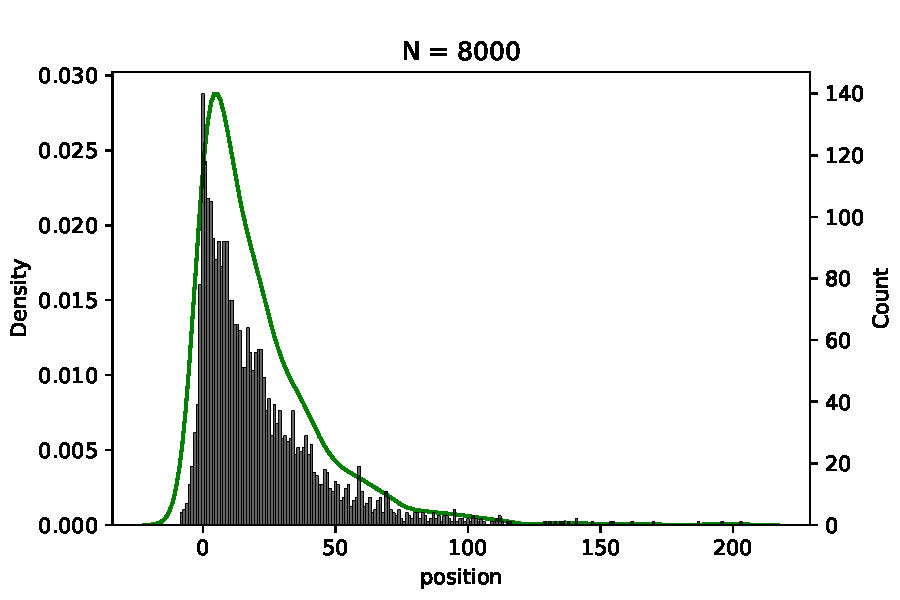
\includegraphics[scale = 0.45]{reset_8000.pdf}
    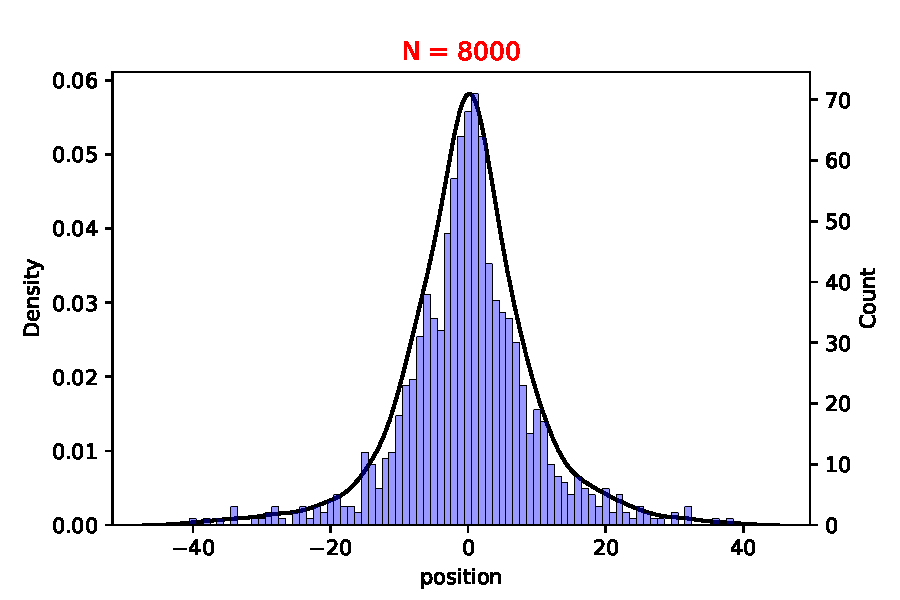
\includegraphics[scale = 0.55]{reset_8000_sym.pdf}
    \caption{Walker with resetting for $p_r = 0.3$.Defined for symmetric walker with $p = q = 0.5$. As expected, we see a spike and at peak we can observe the plot no longer remains differentiable.}
    \label{fig:my_label}
\end{figure}



\begin{figure}[H]
    \centering
    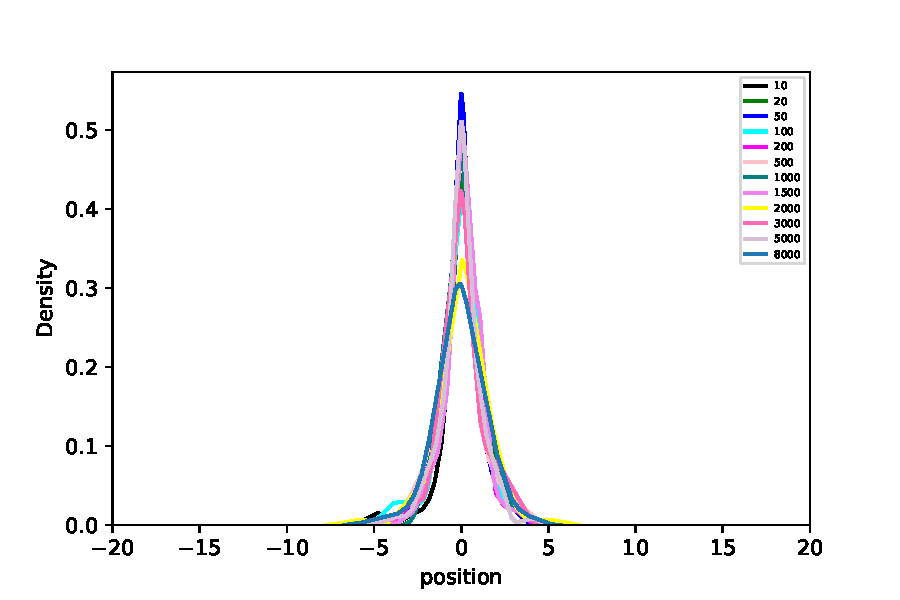
\includegraphics[scale = 0.5]{universal.pdf}
    \caption{Position distribution of walker for different number of steps. We observe that plots start to overlap with increment in number of steps. ($p$,$q$) and resetting are defined for probability $0.6$ and $0.4$ respectively and $p_r = 0.3$. }
    \label{fig:my_label}
\end{figure}


We already saw in Fig. 7 that after a certain number of steps, the position distribution continues to remain invariant under time. Since the PDF is independent of time, moments of the walker should also be. We confirm this result by observing the mean squared displacement (MSD) of the walker. Thus, for a large number of steps, we should obtain a plot that reflects to this above-mentioned fact. Fig. 8 indeed refers to this observation. 



%This hints to the fact that walker is essentially confined around the origin most of the time. If one considers a target which is near the origin, there is a higher probability that the walker will find the target in finite time. This measure of time is known as the first passage time and will be a central goal for future study.

\section{Conclusion}
{
In this report, we 
reviewed the problem of a simple random walker and learned that the position distribution of the walker is given by the Binomial Distribution. We discussed the results for symmetric as well as biased walkers. The mean displacement is given by $N(p-q)$ which explains centering of the peak around $0$ for symmetric ($p=q$) and shift for biased one ($p \neq q$) respectively.
}
{
In the second part of the report, we introduced the concept of a resetting walker. Interestingly, we observed that the position distribution attains to a time-independent form after a large number of steps. We confirmed it numerically. This was also confirmed with the fact that the MSD saturates to a threshold (plateau) value after certain steps. This naturally reinstates the fact that a saturating MSD may imply a steady state (time independent state) which is indeed the case here. As a future goal, we would like to delve deeper into the first passage time statistics and show explicitly how the knowledge gained here can be utilized to predict many statistical metrics such as the mean, variance of the search time.
}


\begin{figure}[t]
    \centering
    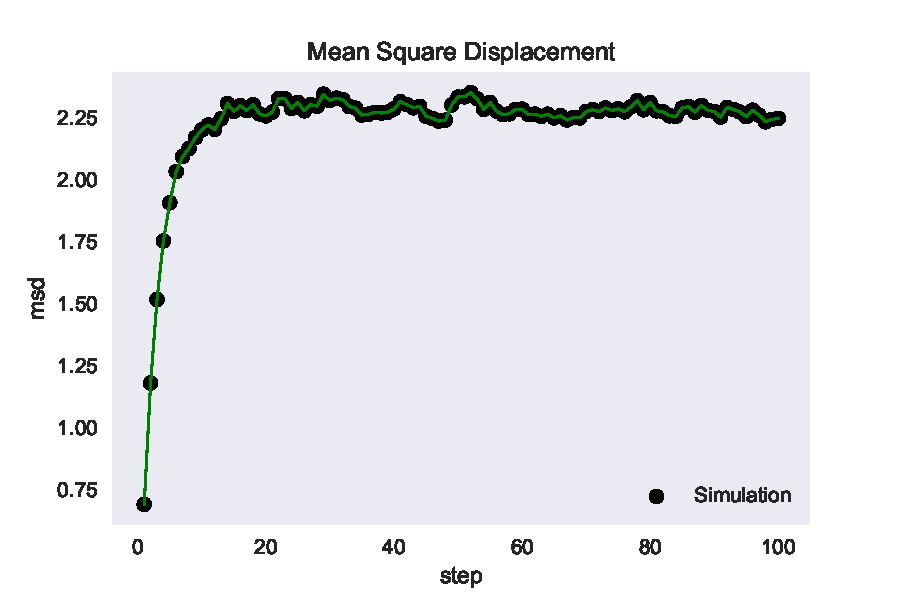
\includegraphics[scale = 0.5]{msd_new.pdf}
    \caption{MSD of a random walker in the presence of resetting as a function of steps. $p$ and $q$ defined for the walker are $0.6$ and $0.4$ respectively and $p_r = 0.3$ .}
    \label{fig:my_label}
\end{figure}













% \caption{Random walker in a discrete time space}


%  Before we proceed, it will be useful to introduce the notations used throughout the paper. We will use $P_X(x)$, $\langle X \rangle$, $\sigma_X ^2$, and $G_X(z) \equiv \langle z^X \rangle$ to denote, respectively, the probability mass/density function (PMF/PDF), mean/expectation, variance, and the probability generating function (PGF) of a discrete random variable $X$ taking values in the non-negative integers. In addition, the survival function and its corresponding generating function for the underlying process are denoted by $Q_{N}(n)$ and $G_{Q_N}(z)$ respectively. In the presence of restart, generating function for the survival function will be denoted by $G_{Q_{N_R}}(z)$.
%  %was recently studied by Montero and Villarroel in \textit{PRE} \textbf{94}, 032132 (2016). 



% \subsection{Review of random walk}
% \label{FPUR}

% \bea
% N_{R}=\begin{cases}
% N & N < R\\
% R+N'_{R} & N \geq R, \label{Renewal eq}
% \end{cases}
% \eea 


% \subsection{Mean}



% \subsection{Generating function for the restarted process}


% \bea 
% G_{N_R}(z) \equiv \left\langle z^{N_R}\right\rangle = \sum_{n=0}^{\infty} P_{N_R}(n)z^{n}, \label{PGF def}
% \eea 
% where $P_{N_R}(n)$ is the probability mass function of $N_R$. 


% \begin{figure}[b]
% 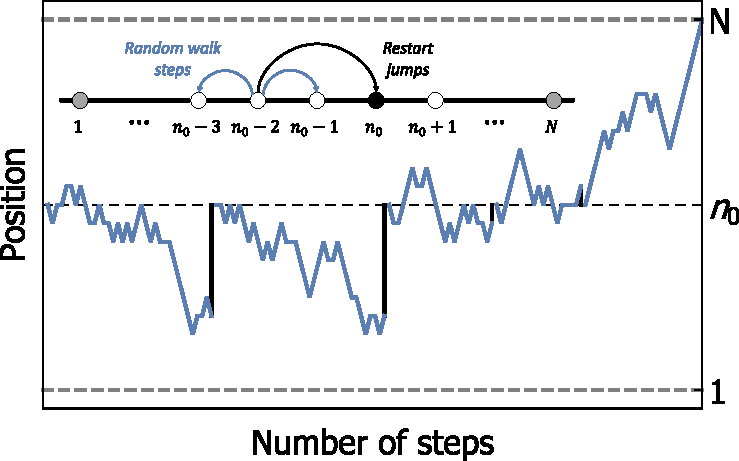
\includegraphics[scale=0.65]{SchematicPanelmainV1.pdf}
% \caption{Schematic of a lattice random walker in a 1D confined geometry under discrete restart. First passage occurs as soon as the walker reaches one of the boundaries located at $1$ and $N$. The restart coordinate is $n_0$, same as the initial condition.}
% \label{Schematic}
% \end{figure}

% \section{Concluding perspective}
% In this note, we presented a simple, and completely general recipe to study statistical properties of discrete first passage processes under arbitrary discrete restart steps. The stages of the computation are as follows:

% \begin{itemize}
%     \item \textbf{Survival functions:} compute the survival functions $Q_N(n)$ and $Q_R(n)$ from the given first passage and restart time distributions namely $P_N(n)$ and $P_R(n)$ respectively [use Eqs. (\ref{Survival N}) and (\ref{Survival R})].
%     \item \textbf{Mean completion time under restart:} next, compute $\text{Pr}(N<R)$ and its complementary probability $\text{Pr}(N \geq R)$ using \eref{denominator}. The mean completion time can then be obtained from \eref{mean FPUR}.
%     \item \textbf{Generating function of the restarted first passage process:} compute the generating functions for the random variable $N_{min}$ and $R_{min}$ and plug in \eref{PGF final result} to derive the generating function for the restarted process from which all the moments can be derived. In some cases, the first passage time density of the compound process can be obtained making use of \eref{PGF PMF}. This was demonstrated in \cite{RW1}. \\
% \end{itemize}


% \noindent
% \textbf{Numerical treatment.---} 



% \begin{acknowledgments}

% \end{acknowledgments}

 \begin{thebibliography}{1}
 
 
 \bibitem{LRW-4}
 Klafter, J. and Sokolov, I.M., 2011. First steps in random walks: from tools to applications. Oxford University Press.

 \bibitem{FPUR}
 Pal, A. and Reuveni, S., 2017. First passage under restart. Physical review letters, 118(3), p.030603.

 \bibitem{RW1}
 Bonomo, O.L. and Pal, A., 2021. First passage under restart for discrete space and time: Application to one-dimensional confined lattice random walks. Physical Review E, 103(5), p.052129.



% \bibitem{LRW-5}

% Rudnick, J. and Gaspari, G., 2004. Elements of the random walk: an introduction for advanced students and researchers. Cambridge University Press.


% \bibitem{Restart1}
% Evans, M.R. and Majumdar, S.N., 2011. Diffusion with stochastic resetting. Physical review letters, 106(16), p.160601.

% \bibitem{Restart-review}
% Evans, M.R., Majumdar, S.N. and Schehr, G., 2020. Stochastic resetting and applications. Journal of Physics A: Mathematical and Theoretical, 53(19), p.193001.


% \bibitem{interval1}
% Pal, A. and Prasad, V.V., 2019. First passage under stochastic resetting in an interval. Physical Review E, 99(3), p.032123.

% \bibitem{interval2}
% Pal, A. and Prasad, V.V., 2019. Landau-like expansion for phase transitions in stochastic resetting. Physical Review Research, 1(3), p.032001.

% % \bibitem{PalJphysA}  Pal, A., Kundu, A. and Evans, M.R., 2016. Diffusion under time-dependent resetting. Journal of Physics A: Mathematical and Theoretical, 49(22), p.225001.

\end{thebibliography}
 
\end{document}




